%! alt Triangle ABC with AB = 6, AC = 10 and BC = 8 times root 5 minus 8, about 9.89. The bisector from A meets BC at D. A circle through A touches BC at D and crosses AB at P and AC at Q. The chord PQ is parallel to BC and passes through the incentre I, so I and PQ are at the same height above BC.
%! after_paragraph 2
%! scale 1/2
%! let S = sqrt(5)
%! let H = sqrt(30*sqrt(5) - 34)
%! let G = (sqrt(5) - 1)/2
% The shared preamble of every Cevian figure. pipeline/figures turns these colours into theme-aware paint,
% and refuses any other colour, so draw only with them:
%   figink (lines and labels), figaux (construction lines), figaccent (the object the argument turns on),
%   figtint and figaccenttint (light fills).
\documentclass[border=1.5pt]{standalone}
\usepackage{tkz-euclide}
\definecolor{figink}{RGB}{0,0,0}
\definecolor{figaux}{RGB}{85,85,85}
\definecolor{figaccent}{RGB}{192,57,43}
\definecolor{figtint}{RGB}{221,221,221}
\definecolor{figaccenttint}{RGB}{245,213,208}
% tkz-euclide's defaults draw circles, compasses and marks in 50% grey and fill points with a tint.
\makeatletter
\def\tkz@otherlinecolor{figink}
\def\tkz@euc@circlecolor{figink}
\def\tkz@euc@compasscolor{figink}
\def\tkz@euc@mkcolor{figink}
\def\tkz@mk@fill{figink}
\def\tkz@euc@pointfillcolor{figink}
\makeatother
\tkzSetUpLine[color=figink,line width=.7pt]
\tkzSetUpArc[color=figink,line width=.7pt]
\tkzSetUpCompass[color=figink,line width=.5pt]
\tkzSetUpPoint[color=figink,fill=figink,size=3.1pt]
\tikzset{
  every picture/.style={line cap=round,line join=round,color=figink},
  circle style/.append style={color=figink,line width=.7pt},
  aux/.style={color=figaux,line width=.45pt,dash pattern=on 2.6pt off 2pt},
  key/.style={color=figaccent,line width=1pt},
  mk/.style={color=figink,line width=.5pt},
  lbl/.style={color=figink,inner sep=2.2pt},
  len/.style={color=figink,inner sep=1.5pt,font=\small},
}

\begin{document}
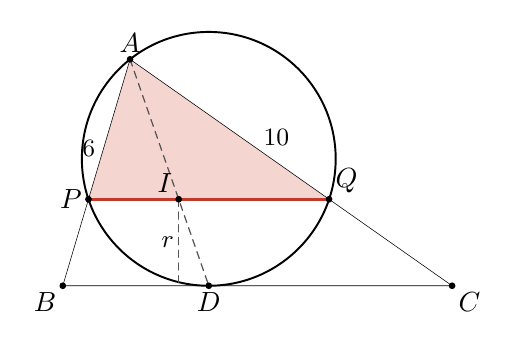
\begin{tikzpicture}
\tkzDefPoint(0.0,0.0){B} %! B = (0, 0)
\tkzDefPoint(4.9442719,0.0){C} %! C = (8*S - 8, 0)
\tkzDefPoint(0.85410197,2.8758494){A} %! A = (3*S - 5, H)
\tkzDefPoint(1.8541020,0.0){D} %! D = (3*S - 3, 0)
\tkzDefPoint(1.8541020,1.6117864){O} %! O = (3*S - 3, 15*(S - 1)/H)
\tkzDefPoint(0.32623792,1.0984767){P} %! P = lerp(A, B, G)
\tkzDefPoint(3.3819660,1.0984767){Q} %! Q = lerp(A, C, G)
\tkzDefPoint(1.4721360,1.0984767){I} %! I = incentre(A, B, C)
\tkzDefPoint(1.4721360,0.0){J} %! J = foot(I, B, C)
%! fact dist(A, B) == 6
%! fact dist(A, C) == 10
%! fact equal(dist(B, C), sqrt(320) - 8)
%! fact equal(angle(B, A, D), angle(D, A, C))
%! fact on_segment(D, B, C)
%! fact on_segment(P, A, B)
%! fact on_segment(Q, A, C)
%! fact on_circle(A, O, dist(O, D))
%! fact on_circle(P, O, dist(O, D))
%! fact on_circle(Q, O, dist(O, D))
%! fact perp(O, D, B, C)
%! fact parallel(P, Q, B, C)
%! fact collinear(I, P, Q)
%! fact collinear(I, A, D)
%! fact equal(dist(I, J), inradius(A, B, C))
%! fact equal(y(P), y(I))
\tkzFillPolygon[color=figaccenttint](A,P,Q)
\tkzDrawCircle(O,D)
\tkzDrawSegment[aux](A,D)
\tkzDrawPolygon(A,B,C)
\tkzDrawSegment[aux](I,J)
\tkzDrawSegment[key](P,Q)
\tkzDrawPoints(A,B,C,D,P,Q,I)
\tkzLabelPoint[above,lbl](A){$A$}
\tkzLabelPoint[below left,lbl](B){$B$}
\tkzLabelPoint[below right,lbl](C){$C$}
\tkzLabelPoint[below,lbl](D){$D$}
\tkzLabelPoint[left,lbl](P){$P$}
\tkzLabelPoint[above right,lbl](Q){$Q$}
\tkzLabelPoint[above left,lbl](I){$I$}
\tkzLabelSegment[left,pos=.5,len](I,J){$r$}
\tkzLabelSegment[above left,pos=.55,len](B,A){$6$}
\tkzLabelSegment[above right,pos=.4,len](A,C){$10$}
\end{tikzpicture}
\end{document}
